\appendix
\chapter{Appendix}
\section*{Beschreibung der Erfindung \ref{beschPDF}}
\section*{Schutzansprüche \ref{schutzPDF}}
\section*{Zusammenfassung \ref{zusammenfassungPDF}}
\section*{Code für Schutzanspruch 3 \ref{lst:schutz3}}
\section*{Code für Schutzanspruch 4 \ref{lst:schutz4}}
\section*{Code für Schutzanspruch 9 \ref{lst:schutz9}}
\section*{Code für Schutzanspruch 10 \ref{lst:schutz10}}
\pagestyle{plain}
\centering
% Add the entry to the ToC for "Beschreibung der Erfindung"
\phantomsection
\addcontentsline{toc}{section}{Beschreibung der Erfindung}
\label{beschPDF} 
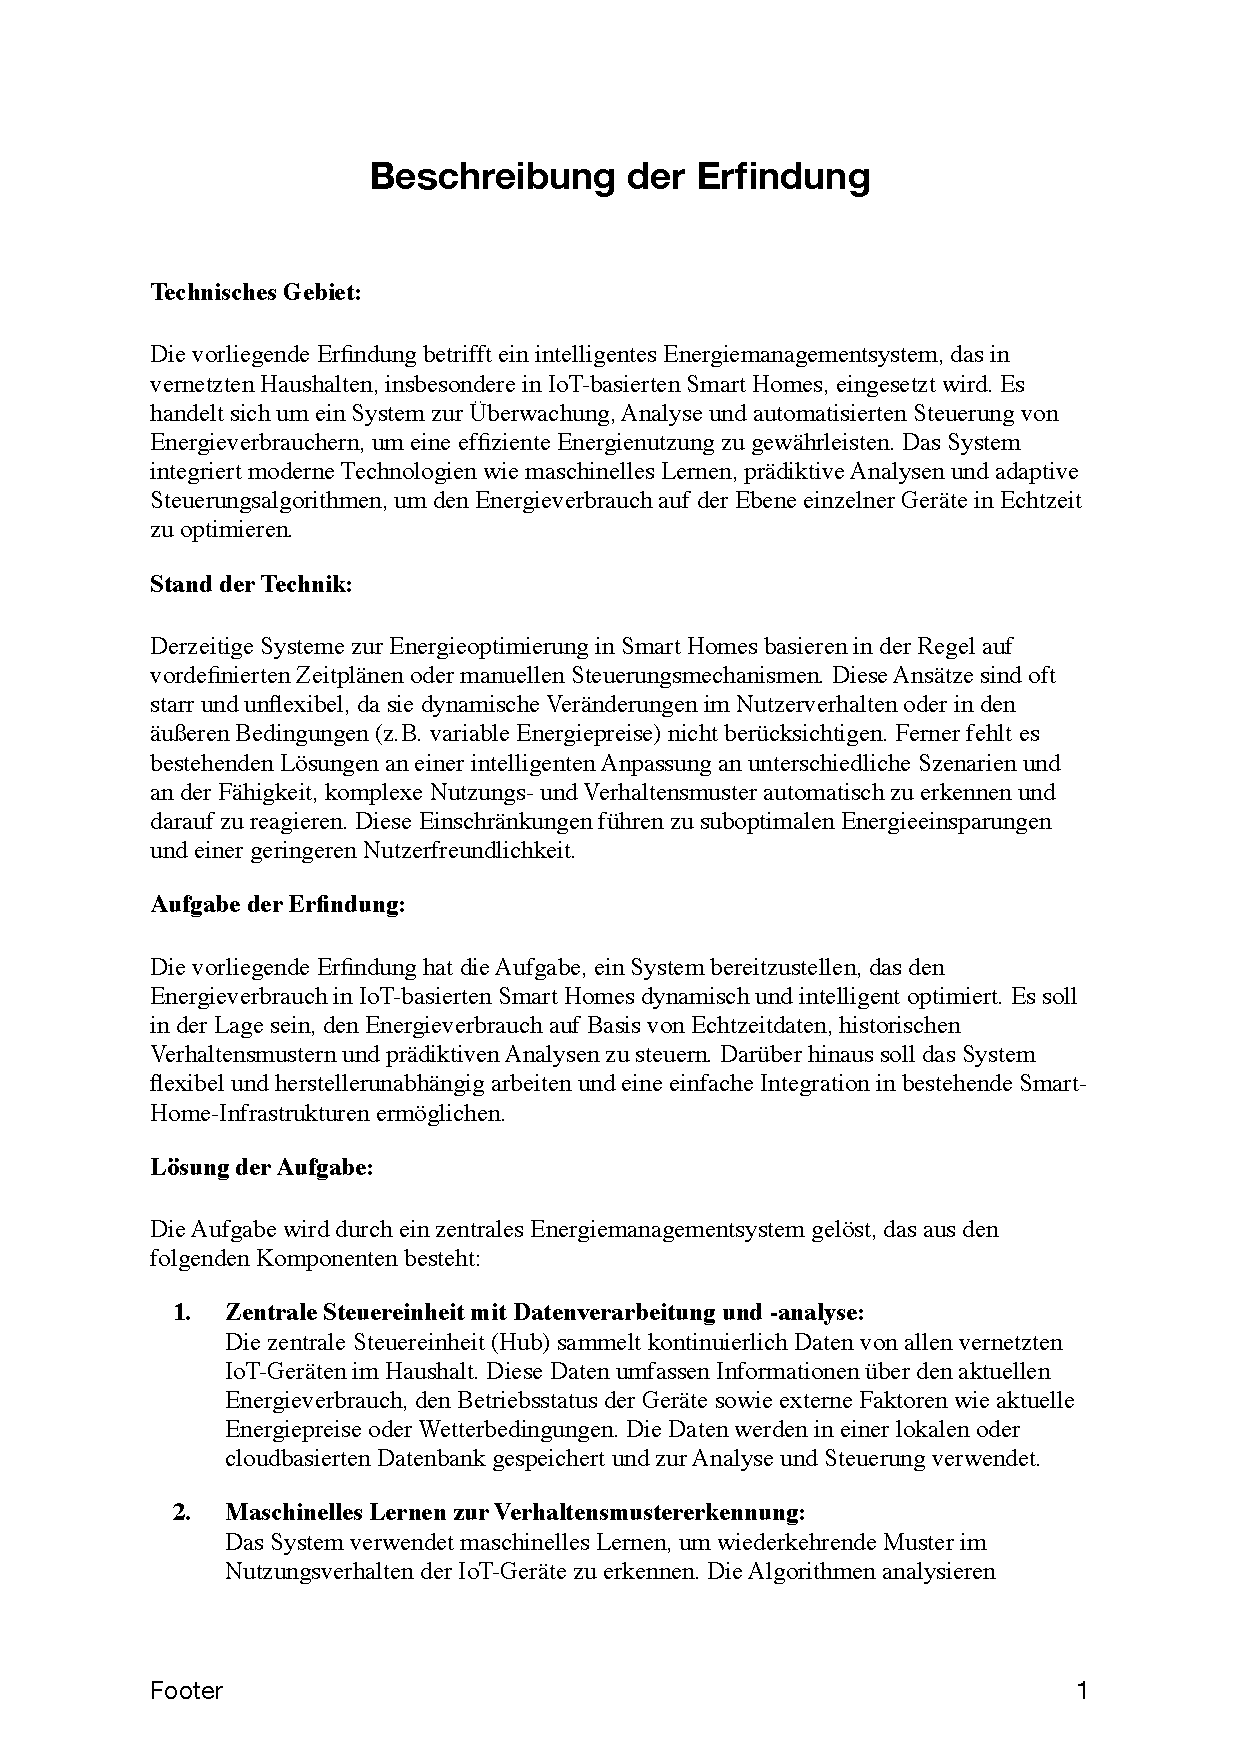
\includepdf[pages={1-3},pagecommand={\thispagestyle{empty}},offset=0 -2cm]{Beschreibung der Erfindung.pdf}
% Add the entry to the ToC for "Schutzansprüche"
\phantomsection
\addcontentsline{toc}{section}{Schutzansprüche}
\label{schutzPDF} 
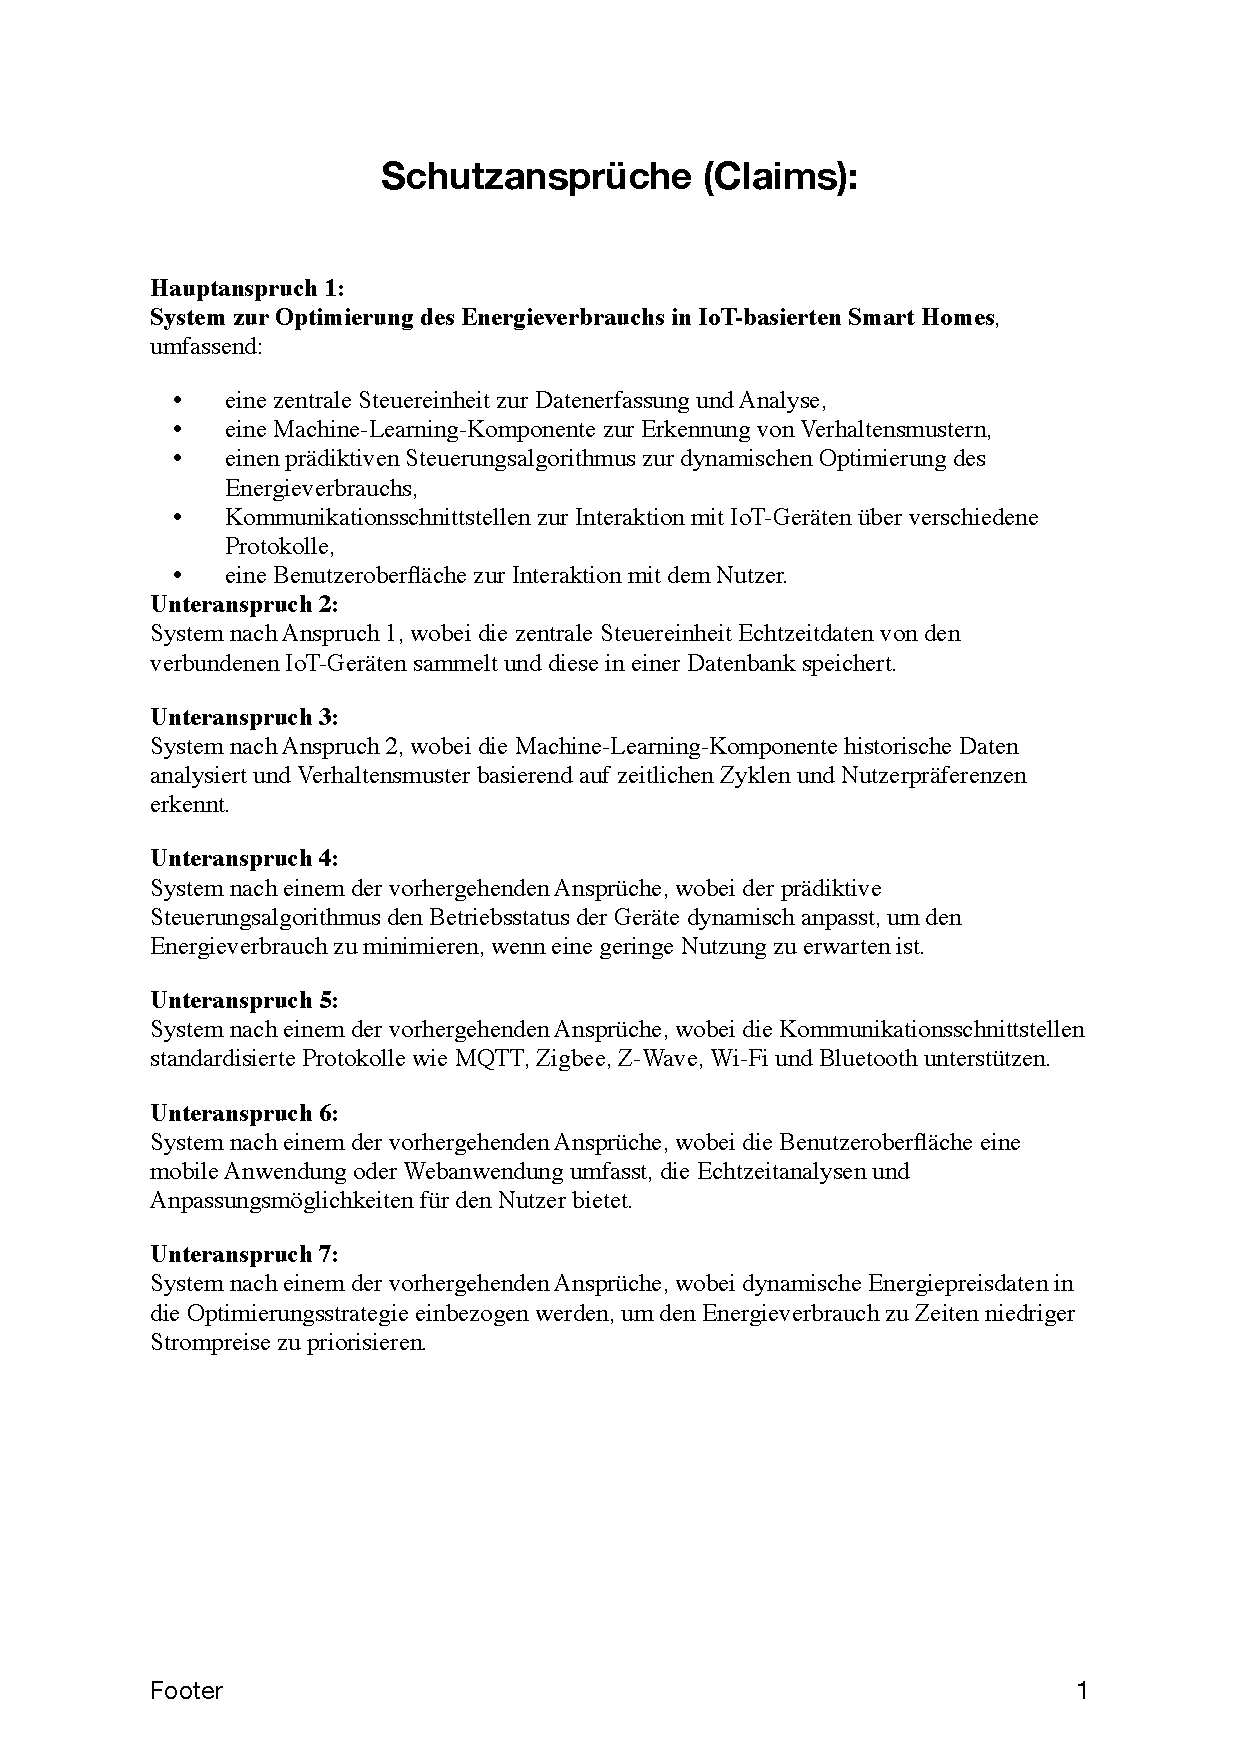
\includepdf[pages={1-2},pagecommand={\thispagestyle{empty}},offset=0 -2cm]{Schutzansprueche.pdf}

% Add the entry to the ToC for "Zusammenfassung"
\phantomsection
\addcontentsline{toc}{section}{Zusammenfassung}
\label{zusammenfassungPDF}  
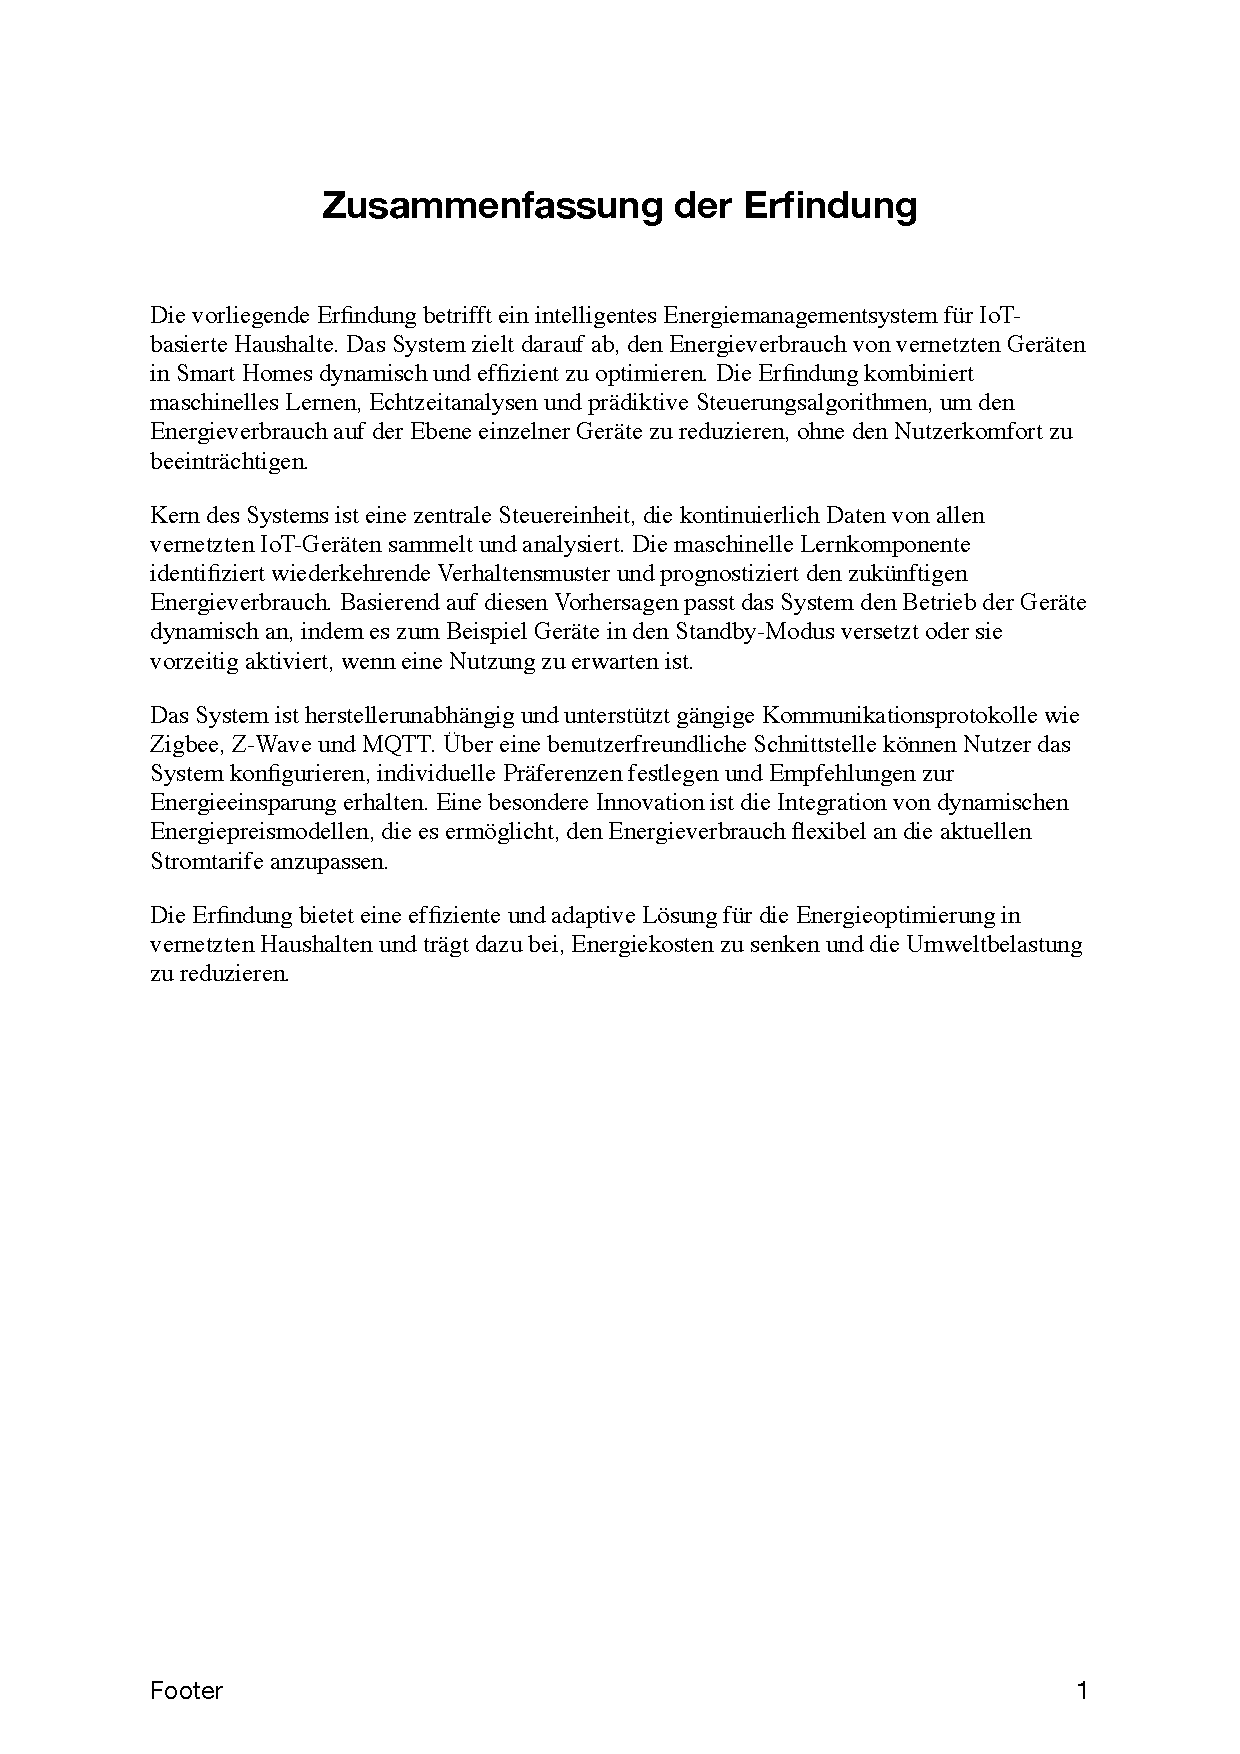
\includepdf[pages={1},pagecommand={\thispagestyle{empty}},offset=0 -2cm]{Zusammenfassung.pdf}



\lstset{language=Python,
        basicstyle=\ttfamily\footnotesize,
        breaklines=true,
        numbers=left,
        stepnumber=1,
        numberstyle=\tiny,
        frame=single,
        caption={Python Code},
        literate=%
            {Ö}{{\"O}}1
            {Ä}{{\"A}}1
            {Ü}{{\"U}}1
            {ß}{{\ss}}1
            {ü}{{\"u}}1
            {ä}{{\"a}}1
            {ö}{{\"o}}1
            {~}{{\textasciitilde}}1
}

\phantomsection
\addcontentsline{toc}{section}{Code Schutzanspruch 3 }
\begin{lstlisting}[language=python,caption=Code für Schutzanspruch 3, label=lst:schutz3]
# Code for Schutzanspruch 3
import pandas as pd
from sklearn.ensemble import RandomForestRegressor
from sklearn.model_selection import train_test_split
from sklearn.metrics import mean_squared_error
import numpy as np
import matplotlib.pyplot as plt

# Beispielhafte historische Verbrauchsdaten (Stundenweise)
data = {
    "timestamp": pd.date_range(start="2024-01-01", periods=1000, freq="H"),
    "power_consumption": np.random.normal(loc=100, scale=10, size=1000)  # Verbrauchsdaten simuliert
}

# Umwandlung in ein DataFrame
df = pd.DataFrame(data)

# Extrahieren von Merkmalen aus dem Zeitstempel (z.B. Stunde, Wochentag, Tag)
df['hour'] = df['timestamp'].dt.hour
df['day_of_week'] = df['timestamp'].dt.dayofweek
df['day_of_month'] = df['timestamp'].dt.day

# Eingabevariablen (Merkmale) und Zielvariable (Verbrauch) definieren
X = df[['hour', 'day_of_week', 'day_of_month']]  # Merkmale
y = df['power_consumption']  # Zielvariable (Verbrauch)

# Daten in Trainings- und Testdaten aufteilen
X_train, X_test, y_train, y_test = train_test_split(X, y, test_size=0.2, random_state=42)

# Machine-Learning-Modell: Random Forest Regressor
model = RandomForestRegressor(n_estimators=100, random_state=42)

# Modell mit den Trainingsdaten trainieren
model.fit(X_train, y_train)

# Vorhersagen für den Testdatensatz machen
y_pred = model.predict(X_test)

# Berechnung des Fehlers (Mean Squared Error)
mse = mean_squared_error(y_test, y_pred)
print(f"Mean Squared Error: {mse:.2f}")

# Ergebnisse visualisieren
plt.figure(figsize=(10, 6))
plt.plot(y_test.values, label='Tatsächlicher Verbrauch', color='blue')
plt.plot(y_pred, label='Vorhergesagter Verbrauch', color='orange')
plt.title("Vergleich von tatsächlichem und vorhergesagtem Energieverbrauch")
plt.xlabel("Zeitpunkt (Index)")
plt.ylabel("Verbrauch (kWh)")
plt.legend()
plt.show()

# Vorhersage für einen zukünftigen Zeitraum
future_hours = pd.DataFrame({
    "hour": [8, 12, 18, 22],  # Beispielstunden
    "day_of_week": [1, 1, 1, 1],  # Angenommener Wochentag
    "day_of_month": [15, 15, 15, 15]  # Angenommener Tag des Monats
})

# Vorhersage des zukünftigen Energieverbrauchs
future_predictions = model.predict(future_hours)
print("Vorhersage für zukünftigen Energieverbrauch:")
for i, pred in enumerate(future_predictions):
    print(f"Stunde {future_hours['hour'][i]}: {pred:.2f} kWh")
    
\end{lstlisting}




\phantomsection
\addcontentsline{toc}{section}{Code Schutzanspruch 4 }
\begin{lstlisting}[language=python,caption=Code für Schutzanspruch 4, label=lst:schutz4]
# Code for Schutzanspruch 4
import datetime
import numpy as np
import pandas as pd
from sklearn.ensemble import RandomForestRegressor
import random

# Beispielhafte Daten für Energieverbrauch (in Watt)
# In einem echten System stammen diese Daten von IoT-Geräten
historical_data = pd.DataFrame({
    'hour': list(range(24)),  # Stunden des Tages
    'energy_consumption': [random.randint(50, 200) for _ in range(24)]  # Zufälliger Energieverbrauch
})

# IoT-Gerüte und deren Status (ein/aus)
devices = {
    'smart_light': {'status': 'off', 'power': 10},
    'thermostat': {'status': 'off', 'power': 200},
    'washing_machine': {'status': 'off', 'power': 500},
}

# Machine-Learning-Modell: RandomForest zur Vorhersage des Energieverbrauchs
def train_model(data):
    # Trainingsdaten: Stunde des Tages und Energieverbrauch
    X = data[['hour']]
    y = data['energy_consumption']
    
    # Modell erstellen und trainieren
    model = RandomForestRegressor(n_estimators=100)
    model.fit(X, y)
    
    return model

# Modell basierend auf historischen Daten trainieren
model = train_model(historical_data)

# Prädiktive Funktion zur Vorhersage des Energieverbrauchs basierend auf der aktuellen Stunde
def predict_energy_consumption(current_hour):
    return model.predict([[current_hour]])[0]

# Steuerungsalgorithmus zur Anpassung der Gerätestatus basierend auf Vorhersagen
def optimize_device_status():
    current_hour = datetime.datetime.now().hour  # Aktuelle Stunde
    predicted_usage = predict_energy_consumption(current_hour)
    
    # Beispielhafter Schwellwert: Wenn Vorhersage > 150 Watt, schalte Geräte aus
    threshold = 150
    
    print(f"Vorhergesagter Energieverbrauch für Stunde {current_hour}: {predicted_usage:.2f} Watt")
    
    if predicted_usage > threshold:
        for device in devices:
            devices[device]['status'] = 'off'
            print(f"{device} ausgeschaltet.")
    else:
        for device in devices:
            devices[device]['status'] = 'on'
            print(f"{device} eingeschaltet.")
    
    return devices

# Ausführung des Optimierungsalgorithmus
optimized_devices = optimize_device_status()

# Ausgabe des aktuellen Gerätestatus
print("\nAktueller Gerätestatus:")
for device, info in optimized_devices.items():
    print(f"{device}: {info['status']}, Energieverbrauch: {info['power']} Watt")

\end{lstlisting}

\phantomsection
\addcontentsline{toc}{section}{Code Schutzanspruch 9 }
\begin{lstlisting}[language=python,caption=Code für Schutzanspruch 9, label=lst:schutz9]
# Code for Schutzanspruch 9
import pandas as pd
import numpy as np
from sklearn.ensemble import RandomForestRegressor
from sklearn.model_selection import train_test_split
from sklearn.metrics import mean_squared_error

# Simulierte Daten
# Spalten: Zeitstempel, Energieverbrauch, Energiepreis, Wetterbedingungen
data = {
    "timestamp": pd.date_range(start="2024-01-01", periods=1000, freq="H"),
    "energy_consumption": np.random.randint(50, 300, size=1000),
    "energy_price": np.random.uniform(0.10, 0.30, size=1000),
    "temperature": np.random.uniform(-10, 35, size=1000)  # Beispielhafte Wetterbedingung
}

# Erstellen eines DataFrames
df = pd.DataFrame(data)

# Feature-Engineering: Extrahieren von Zeitinformationen
df['hour'] = df['timestamp'].dt.hour
df['day'] = df['timestamp'].dt.dayofweek
df['month'] = df['timestamp'].dt.month

# Definieren der Eingabe- und Ausgabedaten
X = df[['hour', 'day', 'month', 'energy_price', 'temperature']]
y = df['energy_consumption']

# Aufteilen der Daten in Trainings- und Testdatensatz
X_train, X_test, y_train, y_test = train_test_split(X, y, test_size=0.2, random_state=42)

# Modelltraining mit RandomForest
model = RandomForestRegressor(n_estimators=100, random_state=42)
model.fit(X_train, y_train)

# Vorhersage des Energieverbrauchs
y_pred = model.predict(X_test)

# Evaluierung des Modells
mse = mean_squared_error(y_test, y_pred)
print(f"Mean Squared Error: {mse}")

# Beispielhafte Vorhersage für einen neuen Datenpunkt
new_data = np.array([[14, 2, 3, 0.15, 22]])  # 14 Uhr, Dienstag, März, Energiepreis 0.15, 22 Grad
predicted_consumption = model.predict(new_data)
print(f"Vorhergesagter Energieverbrauch: {predicted_consumption[0]} kWh")
\end{lstlisting}


\phantomsection
\addcontentsline{toc}{section}{Code Schutzanspruch 10 }
\begin{lstlisting}[language=python,caption=Code für Schutzanspruch 10, label=lst:schutz10]
# Code for Schutzanspruch 10
import time
from random import randint

class IoTDevice:
    def __init__(self, name, power_usage, critical=False):
        self.name = name
        self.power_usage = power_usage
        self.status = "off"  # Device starts off
        self.critical = critical  # Critical devices stay on longer

    def turn_on(self):
        if self.status == "off":
            self.status = "on"
            print(f"{self.name} is now ON.")
    
    def turn_off(self):
        if self.status == "on":
            self.status = "off"
            print(f"{self.name} is now OFF.")
    
    def standby(self):
        if self.status == "on":
            self.status = "standby"
            print(f"{self.name} is now in STANDBY mode.")

# Define a list of IoT devices
devices = [
    IoTDevice("Smart Light", power_usage=10),
    IoTDevice("Thermostat", power_usage=200, critical=True),
    IoTDevice("Washing Machine", power_usage=500),
    IoTDevice("Air Conditioner", power_usage=1500),
    IoTDevice("Laptop", power_usage=50)
]

# Function to optimize energy consumption
def optimize_energy():
    for device in devices:
        # Random energy need simulation
        energy_need = randint(0, 100)
        print(f"Checking {device.name} (Current status: {device.status}, Energy need: {energy_need})")
        
        if energy_need < 30:
            device.turn_off()
        elif 30 <= energy_need < 70:
            if not device.critical:
                device.standby()
            else:
                device.turn_on()
        else:
            device.turn_on()
        time.sleep(1)  # Simulate real-time processing

# Simulate energy optimization
print("Starting energy optimization process...")
while True:
    optimize_energy()
    print("Optimization round complete. Rechecking in 10 seconds...\n")
    time.sleep(10)
\end{lstlisting}